\documentclass{beamer}
\mode<presentation>
{
\usetheme{default}
%\usetheme{Hannover}
%\usetheme{Boadilla}
}

\usefonttheme[onlymath]{serif}


\usepackage[lined,boxed,commentsnumbered]{algorithm2e}
\usepackage{epsfig}
\usepackage{amssymb}
\usepackage{amsthm}
\usepackage{latexsym}
\usepackage{amsfonts}
\usepackage{graphicx}
\usepackage{amsmath}
\usepackage{color}
\usepackage{graphicx}
\usepackage{psfrag}
%\usepackage{multirow}


%\renewcommand{\multirowsetup}{\centering}


\newtheorem{thm}{Theorem}
\newtheorem{prop}{Proposition}

\newcommand{\indic}{\mathbb{I}}
\newcommand{\esp}{\mathbb{E}}
\newcommand{\proba}{\mathbb{P}}
\newcommand{\nn}{\mathbb{N}}
\newcommand{\rr}{\mathbb{R}}
\newcommand{\zz}{\mathbb{Z}}
\newcommand{\Num}{N_U(\mot)}
\newcommand{\Nm}{N(\mot)}
\newcommand{\Yu}{Y_U}
\newcommand{\Extu}{Ext_U}
\newcommand{\mot}{\mathbf{m}}
\newcommand{\argmax}{\mathrm{argmax}}

\DeclareMathOperator{\covmat}{{\bf S}}
\DeclareMathOperator{\bZ}{{\bf Z}}
\DeclareMathOperator{\tZ}{\tilde{Z}}
\DeclareMathOperator{\btZ}{\tilde{\bZ}}
\DeclareMathOperator{\bI}{{\bf I}}
\DeclareMathOperator{\bi}{{\bf i}}
\DeclareMathOperator{\bn}{{\bf n}}
\DeclareMathOperator{\bm}{{\bf m}}
\DeclareMathOperator{\bX}{{\bf X}}
\DeclareMathOperator{\bx}{{\bf x}}
\DeclareMathOperator{\bY}{{\bf Y}}
\DeclareMathOperator{\bG}{{\bf G}}
\DeclareMathOperator{\bg}{{\bf g}}
\DeclareMathOperator{\bK}{{\bf K}}
\DeclareMathOperator{\Dirichlet}{Dir}
\DeclareMathOperator{\bA}{\bf A}
\DeclareMathOperator{\bb}{\bf b}
\DeclareMathOperator{\bB}{\bf B}
\DeclareMathOperator{\bW}{{\bf W}}
\DeclareMathOperator{\tW}{\tilde{W}}
\DeclareMathOperator{\btW}{\tilde{\bW}}
\DeclareMathOperator{\bM}{{\bf M}}
\DeclareMathOperator{\bU}{{\bf U}}
\DeclareMathOperator{\bu}{{\bf u}}
\DeclareMathOperator{\bV}{{\bf V}}
\DeclareMathOperator{\bv}{{\bf v}}
\DeclareMathOperator{\bC}{{\bf C}}
\DeclareMathOperator{\bc}{{\bf c}}
\DeclareMathOperator{\bP}{{\bf P}}
\DeclareMathOperator{\bD}{{\bf D}}
\DeclareMathOperator{\bE}{{\bf E}}
\DeclareMathOperator{\btE}{\tilde{\bE}}
\DeclareMathOperator{\Beta}{Beta}
\DeclareMathOperator{\Gam}{Gam}
\DeclareMathOperator{\Bernoulli}{\mathcal{B}}
\DeclareMathOperator{\Gaussian}{\mathcal{N}}
\DeclareMathOperator{\LowerBound}{\mathcal{L}}
\DeclareMathOperator{\bdelta}{\boldsymbol{\delta}}
\DeclareMathOperator{\bDelta}{\boldsymbol{\Delta}}
\DeclareMathOperator{\bgamma}{\boldsymbol{\gamma}}
\DeclareMathOperator{\btheta}{\boldsymbol{\theta}}
\DeclareMathOperator{\balpha}{\boldsymbol{\alpha}}
\DeclareMathOperator{\bbeta}{\boldsymbol{\beta}}
\DeclareMathOperator{\bSigma}{\boldsymbol{\Sigma}}
\DeclareMathOperator{\bxi}{\boldsymbol{\xi}}
\DeclareMathOperator{\bpi}{\boldsymbol{\pi}}
\DeclareMathOperator{\bPi}{\boldsymbol{\Pi}}
\DeclareMathOperator{\boeta}{\boldsymbol{\eta}}
\DeclareMathOperator{\bozeta}{\boldsymbol{\zeta}}
\DeclareMathOperator{\btau}{\boldsymbol{\tau}}
\DeclareMathOperator{\bttau}{\tilde{\btau}} 
\DeclareMathOperator{\bmu}{\boldsymbol{\mu}}
\DeclareMathOperator{\bkappa}{\boldsymbol{\kappa}}
\DeclareMathOperator{\KL}{\mathrm{KL}}

\setbeamertemplate{blocks}[rounded][shadow=true]


\title{Etude structurelle des r\'eseaux: mod\`eles al\'eatoires, motifs et cycles}
\author{Etienne Birmel\'e  }
\institute{Universit\'e d'Evry-val-d'Essonne \\ Laboratoire Statistique et G\'enome}
\date{3 novembre 2011}
%\date{}

\AtBeginSection[]
{
\frame{
  \tableofcontents[currentsection,hideothersubsections]
} 
}


\begin{document}
 
\begin{frame}
\titlepage
\vfill
\begin{figure}
  \begin{center}
    \begin{tabular}{ccccc}
     %\begin{figure}
       \epsfig{file=figures/affiliations/sg.eps,width=1.5cm}
     %\end{figure}
    &  %\begin{figure}
      \epsfig{file=figures/affiliations/cnrs.ps,width=1cm}
      %\end{figure}
    &  %\begin{figure}
       \epsfig{file=figures/affiliations/inra.ps,width=1.5cm}
      %\end{figure}
    &   %\begin{figure}
       \epsfig{file=figures/affiliations/inria.ps,width=1.5cm}
      %\end{figure}
    &  %\begin{figure}
       \epsfig{file=figures/affiliations/ueve.ps,width=1.2cm}
      %\end{figure}
    \end{tabular}
  \end{center}
\end{figure}
\end{frame}



\begin{frame}
\frametitle{Context: biological networks}
\begin{figure}
\epsfig{file=figures/networkpage/networkpage.eps, width=1.1\textwidth}
\end{figure}
\end{frame}




\begin{frame}
\frametitle{Context: Statistical analysis of a network's feature}

\begin{enumerate}
\item from biology to graph theory
\item describe the feature of interest in the observed network %(count, enumeration, distribution) 
\uncover<2-3>{
\begin{description}
\item[2.1] count/enumeration algorithm 
\item[2.2] structure for an efficient network exploration: tree-decompositions
\end{description}        
}
\item compare the observed description to random ones 
\uncover<3>{
\begin{description}
\item[3.1] what for a null model?
\item[3.2] build a test
\end{description}
}
\item back to biology 
\end{enumerate}


%%saying something like ``historical order in my implication is structural decomposition -> random model -> statistics -> counting/enumerating `` but will present in the order written here so I will start with some perspectives. 
\end{frame}






\section{Enumerating features}

%\begin{frame}
%\frametitle{Enumeration problems}

%\begin{description}
%\item[subgraph occurrence:] enumerate/count the number of occurences of a small graph $H$ in a graph $G$.\\

%{\tiny \textsc{Koskas et al.}, JOBIM, 2011.}

%\item[chemical organisations:] enumerate closed and self-maintaining sets of metabolic reactions.\\

%{\tiny \textsc{Milreu et al.}, WABI'2010, Lecture Notes in Computer Science/ Lecture Notes in Bioinformatics, 2011.}

%\item[stories:] enumerate maximal DAGs which sources and sinks are contained in a given set of vertices of interest.\\

%{\tiny \textsc{Acu\~na et al.},  Workshop of ICALP Graph Algorithms and Applications, 2011.}

%\end{description}

%\end{frame}





\begin{frame}
\frametitle{Subgraph occurrences}

{\bf Data:} A graph $G$ and a small graph $H$.

{\bf Output:} Count or enumeration of the occurrences of $H$ in $G$.

\vspace{-1cm}
\begin{figure}
\epsfig{file=figures/yeast/subnet.ps, width=.4\textwidth, angle=-90}
\end{figure}
\vspace{-1cm}
\begin{figure}
\begin{tabular}{cc}
\mbox{ contains $31270$ occurrences of the $3$-star} &
\epsfig{file=figures/star.eps, width=.05\textwidth}
\end{tabular}
\end{figure}

{\tiny \textsc{Koskas et al.}, JOBIM, 2011.}

\end{frame}


\begin{frame}
\frametitle{Chemical organizations}

{\bf Data:} A metabolic network.

{\bf Output:} Enumerate the sets of compounds that are closed and self-maintaining. 


\begin{figure}
\epsfig{file=figures/organisation.eps, width=.5\textwidth}
\end{figure}




{\tiny \textsc{Milreu et al.}, WABI'2010, Lecture Notes in Computer Science/ Lecture Notes in Bioinformatics, 2011.}


\end{frame}





\begin{frame}
\frametitle{Metabolic stories}

{\bf Data:} A metabolic network with black and white nodes.

{\bf Output:} Enumerate the maximal DAGs without white sources or sinks. 


\begin{figure}
\epsfig{file=figures/stories.eps, width=.4\textwidth}
\end{figure}






{\tiny \textsc{Acu\~na et al.}, Telling Stories,  Workshop of ICALP Graph Algorithms and Applications, 2011.}



\end{frame}










%%%%%%%%%%%%%%%%%%%%%%%%%%%%%%%%%%%%%%%%%%%%%%%%%%%%%%%%%%%%%%%%%%%%%%%%%%%%%%%%%

\section{Random models}

%\begin{frame}
%\frametitle{simulation VS theory}

%Big samples of independant networks do not exist.
%Comparison to random networks has to be done through one of the following:
%\begin{description}
%\item[simulation] generate a sample by repeating an algorithmic procedure;

%\begin{figure}
%\psfrag{la}{$\Rightarrow$}
%\psfrag{rw}{rewiring model:}
%\epsfig{file=figures/rewiring.eps, width=.7\textwidth}
%\end{figure}


%\item[theory] describe a random graph model and look for the theoretical law of the observation of interest.


%\begin{figure}
%\psfrag{la}{$\Rightarrow$}
%\psfrag{er}{Erd\H{o}s-R\'enyi model:}
%\epsfig{file=figures/erdos.eps, width=.7\textwidth}
%\end{figure}

%\end{description}

%\end{frame}

\begin{frame}
\frametitle{Random models}

\begin{block}{Problem}
Find a trade-off between the fit to real data and theoretical maniability.
\end{block}

\begin{itemize}
\item Erd\H{o}s-R\'enyi model: independant edges but poor fit to real data;

\item Rewiring model: fixed degree distribution but no local density and not analitically tractable.

\item Model based on the projection of a hidden bipartite structure: scale-free distribution but poorly tractable.

{\tiny \textsc{Birmel\'e}, Discrete Applied Mathematics, 2009.}

\end{itemize}

\end{frame}




%\begin{frame}
%\frametitle{}

%\begin{figure}
  %\epsfig{file=figures/yeast/shuffle.ps, width=\textwidth, angle=-90} 
%\end{figure}


%\end{frame}









%\begin{frame}
%\frametitle{Is scale-freeness the holy graal?}


%\only<1>{
%\begin{itemize}
%\item a sample of a scale-free graph is not scale-free (Stumpf {\em et al}, 05); 
%\item the degree distribution is not the only characteristic of biological graphs. 
%\end{itemize}
%}


%\only<2>{
%\begin{block}{Moral}
%\begin{center}
%We need more flexibility to tackle also modularity \\
%$$ \Rightarrow$$ \\
%Relax the scale-freeness condition to a degree heterogeneity condition.
%\end{center}
%\end{block}
%}

%\only<1>{
%\begin{figure}
%    \epsfig{file=figures/yeast/rewiringshuffle.ps, width= .65 \textwidth, angle=-90} 
%\end{figure}
%}



%\end{frame}


%Peut-on dire qqch sur ERGM???????????????







\begin{frame}
\frametitle{Stochastic Block Model}

  \begin{itemize}
    \item A mixture model of Erd\H{o}s-R\'enyi graphs (Nowicki and Snijders, 01)
    \item Each vertex has a hidden class: 
         \begin{itemize}
         \item $\bZ_{i} \sim \mathcal{M}\Big(1, \:\balpha =
        (\alpha_{1}, \alpha_{2}, \dots, \alpha_{Q})\Big)$
        \item $Z_{iq}=1$ : vertex $i$ belongs to class $q$
        \end{itemize}
    \item The edges are drawn independently given the vertex classes: 
        \begin{equation*} 
        X_{ij} |\{Z_{iq}Z_{jl} = 1\} \sim \Bernoulli(\pi_{ql})
      \end{equation*}
  \end{itemize}

\begin{figure}
\begin{tabular}{ccccc}
\epsfig{file=figures/affiliation.eps, width=.2\textwidth} & \qquad & \qquad & \qquad & \epsfig{file=figures/sbmex2.eps, width=.15\textwidth}
\end{tabular}
\end{figure}

\begin{itemize}
\item Estimation of the a-posteriori distribution of $Z_i$ gives a classification method on the vertices.
\end{itemize}

\end{frame}


\begin{frame}
\frametitle{Samples}

\vspace{-1cm}
\begin{figure}
  \epsfig{file=figures/yeast/shuffle.ps, width= .8\textwidth, angle=-90} \\
\end{figure}
\end{frame}




\begin{frame}
\frametitle{Parameter estimation in SBM}

\begin{itemize}
\item  $\log p(\bX|\balpha, \bPi) = \log \left\{\sum_{\bZ} p(\bX, \bZ|\balpha,\bPi)\right\}$ is untractable;
\item  Expectation Maximization (EM) algorithm requires the knowledge of $p(\bZ|\bX, \balpha, \bPi)$, which is again untractable;
\item  Nowicki and Snijders (2001) propose an estimation via Gibbs sampling;
\item  Daudin {\em et al.} (2008) propose a frequentist variationnal EM algorithm combined with an ICL criterion for model selection.
\item Bayesian variationnal EM algorithm, new model selection criterion $ILvb$;


{\tiny \textsc{Latouche, Birmel\'e, Ambroise}, Statistical Modelling, to appear.}


{\tiny \textsc{mixer} R-package, http://cran.r-project.org/ } 
\end{itemize}

\end{frame}


\begin{frame}
\frametitle{OSBM}


\begin{block}{Problem}
  The stochastic block model (SBM) and most existing methods assume that each vertex belongs to a single class
\end{block}

\begin{figure}
 \epsfig{file=figures/Palla.eps, width= .25 \textwidth} \\
 \caption{Palla et al. (06)}
\end{figure}
\end{frame}






%\begin{frame}
%\frametitle{Bayesian approach to SBM}
%
%\begin{itemize}
%\item Bayesian approach;
%\item Variationnal Bayes decomposition:
%    \begin{equation*}
%      \log p(\bX) = \mathcal{L}\left(q\right) + \KL\left(q(\cdot)\:||\:
%        p(\cdot|\bX)\right) 
%    \end{equation*}
%    where 
%    \begin{equation*}
%      \LowerBound(q) =  \sum_{\bZ} \int \int q(\bZ,
%      \balpha, \bPi) \log
%      \left\{\frac{p(\bX,         \bZ,         \balpha,
%          \bPi)}{q(\bZ, \balpha, \bPi)}\right\} d \balpha d \bPi
%    \end{equation*}
%\item Optimisation of $\LowerBound(q)$ among the factorized distribution $q(\bZ, \balpha, \bPi) =  q(\balpha) q(\bPi) q(\bZ)$;
%\item New model selection criterion: $ILvb=\mathcal{L}\left(q\right)$ used as an approximation of $\log p(\bX|Q)$.
%\end{itemize}

%{\tiny \textsc{P. Latouche et al.}, .}



%\end{frame}


%\begin{frame}\frametitle{Overlaps in networks}

%  \begin{block}{Problem}
%   The stochastic block model (SBM) and most existing methods assume that each vertex belongs to a single class
%  \end{block}

%  \begin{figure}
%    \epsfig{file=figures/Palla.eps, width= .3 \textwidth} \\
% \caption{Palla et al. (06)}
%  \end{figure}
%\end{frame}


\begin{frame}
\frametitle{Overlapping Stochastic Block Model}

%\begin{block}
%\begin{itemize}
%\item ??? (Palla, ??);
%\item Mixed Membership Stochastic Block Model (Nowicki and Snijders, 01). 
%\end{itemize}
%\end{block}


\begin{itemize}
\item $Z_{iq}$ independent hidden variables:
     \begin{equation*} 
        \bZ_{i} \sim \prod_{q=1}^{Q} \Bernoulli (Z_{iq};\: \alpha_{q})
        = \prod_{q=1}^{Q} \alpha_{q}^{Z_{iq}} (1 - \alpha_{q})^{1 - Z_{iq}}
     \end{equation*}
 \item $\bX|\bZ$ edges drawn independently : 
      \begin{equation*}
        X_{ij}| \bZ_{i}, \bZ_{j} \sim \Bernoulli \big( X_{ij};\:
        g(a_{\bZ_{i}, \bZ_{j}})\big) 
      \end{equation*}
\item $g(t) = 1/\left(1+\exp(-t)\right)$ is the logistic function
      \begin{equation*}
        a_{\bZ_{i}, \bZ_{j}} = \bZ_{i}^{\intercal} \bW \bZ_{j} +
        \bZ_{i}^{\intercal}\bU + \bV^{\intercal}\bZ_{j} + W^{*}
      \end{equation*}
  \end{itemize}

\end{frame}


\begin{frame}
\frametitle{Overlapping Stochastic Block Model}

 \begin{figure}
    \epsfig{file=figures/osbmexample.eps, width= .5 \textwidth} \\
  \end{figure}

\end{frame}


\begin{frame}
\frametitle{Overlapping Stochastic Block Model}

\begin{itemize}
\item allows overlaps;
\item exhibit a natural {\em junk class} corresponding to vertices having $\bZ_i={\bf 0}$;
\item is invariant under
  \begin{itemize}
   \item class permutation;
   \item inversions ($I_q: \quad Z_{iq} \leftarrow 1 -Z_{iq}, \forall i$ )
  \end{itemize}
\item up to permutations and inversions, the model is generically identifiable.
\end{itemize}


\end{frame}






\begin{frame}
\frametitle{OSBM variational inference}

\begin{equation*}
 \log p(\bX) \geq  \mathcal{L}\left(q\right) \geq \LowerBound(q;\:\bxi)
\end{equation*}

$\LowerBound(q;\:\bxi)$ is then optimized among the factorized distributions
$ $ by optimizing $\bxi$, the $Z_i$'s,  $\alpha$ and  $\tilde{W}$  one after another until convergence. 

\begin{itemize}
\item frequentist variationnal EM algorithm;

{\tiny \textsc{Latouche, Birmel\'e and Ambroise}, Annals of Applied Statistics, 2011.}

\item Bayesian variationnal EM algorithm, model selection criterion $ILosbm$;

{\tiny \textsc{Latouche, Birmel\'e and Ambroise}, Coming soon...}
\end{itemize}





\end{frame}


%\begin{frame}
%\frametitle{OSBM Inference}

% \begin{itemize}
%  \item $\btZ_{i} = (\bZ_{i}, 1)^{\intercal}$
%  \item $\btW = \begin{pmatrix}
%      \bW & \bU \\
%      \bV^{\intercal} & W^{*}
%    \end{pmatrix}$
%  \item $a_{\bZ_{i},\bZ_{j}} = \btZ_{i}^{\intercal}\btW \btZ_{j}$
%  \item Parameter set : $\left\{\balpha, \btW\right\}$
%  \end{itemize}

%\end{frame}












%\begin{frame}\frametitle{Inference}
%  \begin{block}{Local optimization}
%    \begin{itemize}
%    \item $\bxi = \argmax_{\bxi}{\LowerBound(q;\: \bxi)}$
%    \end{itemize}
%  \end{block}
%  \begin{block}{E-step}
%    \begin{itemize}
%    \item $q(Z_{iq}) = \Bernoulli(Z_{iq};\:\tau_{iq})$
%    \end{itemize}
%  \end{block}
%  \begin{block}{M-step}
%    \begin{itemize}
%    \item  $q(\balpha) = \prod_{q=1}^{Q} \Beta(\alpha_{q};\:\eta_{q}^{N},\zeta_{q}^{N})$
%    \item  $q(\btW^{vec}) = \mathcal{N}(\btW^{vec};\: \btW_{N}^{vec}, \covmat_{N})$ 
%    \end{itemize}
%  \end{block}
  
%\end{frame}

%\begin{frame}\frametitle{OSBM Inference}

 % \begin{equation*}
 %     \log p(\bX) \geq \LowerBound(q) \geq \LowerBound(q;\:\bxi)
 %  \end{equation*}

 % \begin{description}
 %   \item[Local optimization] $\bxi = \argmax_{\bxi}{\LowerBound(q;\: \bxi)}$
 %   \item[E-step] $q(Z_{iq}) = \Bernoulli(Z_{iq};\:\tau_{iq})$
 %   \item[M-step]
 %   \begin{itemize}
 %   \item  $q(\balpha) = \prod_{q=1}^{Q} \Beta(\alpha_{q};\:\eta_{q}^{N},\zeta_{q}^{N})$
 %   \item  $q(\btW^{vec}) = \mathcal{N}(\btW^{vec};\: \btW^{vec}_{N}, \covmat_{N})$ 
 %   \end{itemize}
 % \end{description}


  % \begin{itemize}
  %   \item After convergence, $\LowerBound(q;\:\bxi)$ is used as model selection criterion.
  % \end{itemize}
  
%\end{frame}



\begin{frame}\frametitle{Model selection criterion}
%  \begin{itemize} 
%  \item After convergence, use $\LowerBound(q;\: \bxi)$ as an approximation of $\log p(\bX|Q)$
%  \end{itemize}
 
    \begin{multline*}
      IL_{osbm} = \\\sum_{i\neq j}^{N} \left\{\log g(\xi_{ij}) - \frac{\xi_{ij}}{2} + \lambda(\xi_{ij})\xi_{ij}^{2}\right\} + \sum_{q=1}^{Q}\log \bigg\{\frac{\Gamma(\eta_{q}^{0}+\zeta_{q}^{0})\Gamma(\eta_{q}^{N})\Gamma(\zeta_{q}^{N})}{\Gamma(\eta_{q}^{0})\Gamma(\zeta_{q}^{0})\Gamma(\eta_{q}^{N}+\zeta_{q}^{N})}\bigg\} \\
      -\frac{1}{2}\log |\frac{\covmat_{0}}{\covmat_{N}}| - \frac{1}{2}(\btW_{0}^{vec})^{\intercal}\covmat_{0}^{-1}\btW_{0}^{vec} + \frac{1}{2}(\btW_{N}^{vec})^{\intercal}\covmat_{N}^{-1}\btW_{N}^{\intercal} \\
      - \sum_{i=1}^{N}\sum_{q=1}^{Q}\bigg\{\tau_{iq}\log\tau_{iq} + (1-\tau_{iq})\log(1-\tau_{iq})\bigg\}
    \end{multline*}
 
\end{frame}


\begin{frame}
\frametitle{Application to the yeast subnetwork}


\begin{figure}
\epsfig{file=figures/osbm/yeastsubnetworkfig.ps, width=.6\textwidth}
\end{figure}

\end{frame}

% Parler à l'oral de la spécialisation de modèles.



%%%%%%%%%%%%%%%%%%%%%%%%%%%%%%%%%%%%%%%%%%%%%%%%%%%%%%%%%%%%%%%%%%%%%%%%%%%%%%%%%%%%%%%%%%%



\section{Local Motifs}





\begin{frame}
\frametitle{Network motifs}

A {\em motif} is a small graph which is over-represented in a network: it's a candidate to be studied for 
a potential biological meaning.
\smallskip



\begin{figure}
\begin{center}
\psfrag{X}{}
\psfrag{Y}{}
\psfrag{Z}{}
\begin{tabular}{ccc}
\mbox{ feed-forward loop } & \hspace{1cm}  & \mbox{ bi-fan } \\
\epsfig{file=figures/38.eps, width=.2\textwidth} & \hspace{1cm}  & 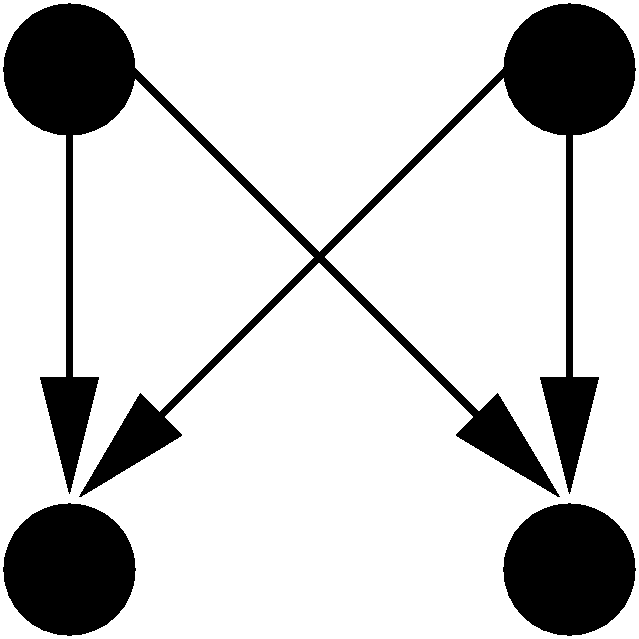
\epsfig{file=figures/bifan.eps, width=.1\textwidth}
\end{tabular}
\end{center}
\end{figure}

%voler figure ffl -> delay à Alon?


\end{frame}






\begin{frame}
\frametitle{Leading ideas}

All previous works (Milo {\em et al} 02, Berg and L\"assig 04, Matias {\em et al} 06, Picard {\em et al} 09) look for an overall over-representation but:

\begin{itemize}
\item A small graph $\mot$  may be over-represented because one of its subgraphs  $\mot'$ is over-represented. 
In that case, $\mot'$ is the relevant motif. 
\item Motifs in regulatory networks are known to be concentrated in very specific places (Lee {\em et al} 02, Dobrin {\em et al} 04).  
\end{itemize}

{\tiny \textsc{Matias et al.}, REVSTAT, 2006.}

\end{frame}




\begin{frame}
\frametitle{ Local motifs}

Consider a pattern $\mot$ and a subgraph $\mot'$ of $\mot$ obtained by the deletion of a vertex in $\mot$.

\begin{figure} [htb] 
\begin{center}
\psfrag{mp}{$\mot'$}
\psfrag{m}{$\mot$}
\epsfig{file=figures/motifex.eps, width=.4\textwidth}
\end{center}
\end{figure}



$\mot$ is a {\em local motif} with respect to $\mot'$ if there exist a {\em theme} (Zhang {\em et al} 2004) of significantly higher order than expected. 
 

\begin{figure} [htb] 
\begin{center}
\psfrag{mp}{$\mot'$}
\epsfig{file=figures/exemple.eps, width=.4\textwidth}
\end{center}
\end{figure}
\end{frame}



\begin{frame}
\frametitle{Random graph model}

We consider a variation of SBM in which the classes are fixed.

Parameters of the model are:
\begin{itemize}
\item a vector of node classes $\{C_1,\ldots ,C_n\}\in \{1,\ldots,Q\}^n$;
\item a connectivity matrix $\Pi$. 
\end{itemize}

The edges are independant and

$$ P(X_{uv}=1 | C_u=q,C_v=l) = \Pi_{ql} $$

\end{frame}


\begin{frame}
\frametitle{Notations}

Let $\mot$ be a pattern on $k$ vertices  and $\mot'$ a subpattern.
Let $U$ be a set of $k-1$ vertices corresponding to an occurence of $\mot'$.
\begin{itemize}
\item $\Num$ is the observed order of the theme;
\item $\lambda_U$ is the expected order of the theme;
\item $\Delta_U=\frac{\Num-\lambda_U}{\lambda_U}$
\end{itemize}


\begin{figure} [htb] 
\begin{center}
\psfrag{U}{$U$}
\psfrag{m1}{$\mot_1$}
\psfrag{m2}{$\mot_2$}
\psfrag{384}{$PDR1$}
\psfrag{388}{$PDR3$}
\psfrag{274}{$PDR5$}
\psfrag{281}{$IPT1$}
\psfrag{300}{$HXT9$}
\psfrag{389}{$HXT11$}
\psfrag{523}{$SNQ2$}
\psfrag{665}{$YOR1$}
\epsfig{file=figures/examplebis.eps, width=.6\textwidth}
\end{center}
\end{figure}

\end{frame}



\begin{frame}
\frametitle{Local bounds on the p-value}

\begin{description}
\item[Concentration inequality]
\end{description}
$ \forall t>0, $
$$
\proba(\Delta_U \geq t) \leq  \proba(G[U] \sim \mot')  e^{-\lambda_U ((1+t)\ln(1+t) -t)} 
$$

\begin{description}
\item[Poisson approximation] 
\end{description}
$ \forall t>1, $
$$
\proba(\Delta_U \geq t) \leq  \proba(G[U] \sim \mot') \frac{\sqrt{t+1}}{\sqrt{2\pi \lambda_U} (t-1)} e^{-\lambda_U ((1+t)\ln(1+t) -t)} 
$$



\end{frame}






\begin{frame}
\frametitle{Multiple testing}

\begin{block}{Multitest problem}
$ \mathcal{O}(n^{k-1})$ positions to consider.
\end{block}

We define
\begin{equation*}\label{gdefinition}
g(\lambda,t) = \lambda \big( (1+t)\log(1+t) -t \big) - \log(\max(1,\frac{\sqrt{t+1}}{\sqrt{2\pi \lambda_U} (t-1)})) 
\end{equation*}
$g(\lambda,.)$ is a one-to-one increasing function and
goes to infinity like $\lambda t \log(t)$.

\begin{eqnarray*}
\mbox{The pattern is a local motif} & \Leftrightarrow & \Num >> \lambda_U \\ 
                              & \Leftrightarrow & \Delta_U >> 0 \\
                              & \Leftrightarrow & g(\lambda_U,\Delta_U) >> 0 
\end{eqnarray*}
\end{frame}


\begin{frame}
\frametitle{A global statistic}


Applying the local theorem to $y$ such that $g(\lambda_U,y)=t$ gives:
\begin{equation*}
 \proba \big(g(\lambda_U,\Delta_U) > t  \big)\leq \proba(G[U]\sim \mot') e^{-t} 
\end{equation*} 

which yields

\begin{thm}\label{main}

Let $N(\mot')$ the random variable counting the number of occurences of $\mot'$. Then, for every $t>0$, 
\begin{equation}
\proba \big(  \max_{U}(g(\lambda_U,\Delta_U))  > t  \big)  \leq  \esp N(\mot')    e^{-t} \label{globaleq}
\end{equation} 

\end{thm}




\end{frame}




\begin{frame}
\frametitle{Filtering procedure}

\only<1>{
\begin{figure} [htb] 
\psfrag{A}{$c$}
\psfrag{B}{$d$}
\psfrag{S}{$a$}
\psfrag{T}{$b$}
\psfrag{u}{$u$}
\psfrag{v}{$v$}
\psfrag{w}{$w$}
\psfrag{petita}{}
\psfrag{petitb}{}
\begin{center}
\epsfig{file=figures/filtering.eps, width=\textwidth}
\end{center}
\label{filteringfig}
\end{figure}
}

\only<2>{
\begin{figure} [htb] 
\psfrag{A}{$c$}
\psfrag{B}{$d$}
\psfrag{S}{$a$}
\psfrag{T}{$b$}
\psfrag{u}{$u$}
\psfrag{v}{$v$}
\psfrag{w}{$w$}
\psfrag{petita}{}
\psfrag{petitb}{}
\begin{center}
\epsfig{file=figures/filtering2.eps, width=\textwidth}
\end{center}
\label{filteringfig}
\end{figure}
}


\end{frame}



\begin{frame}
\frametitle{Local motif detection procedure}

{\bf Data:} a network $G$ , a maximal motif size $k_{max}$, a vector of vertex classes and a connectivity matrix, a threshold $\alpha$.

{\bf Output:} the local motif list.
\bigskip


{\bf Algorithm}

For all motif size $k$ from 2 to $k_{max}$: 

\hspace{.5cm} Enumerate all occurrences of patterns of size $k$.

\hspace{.5cm} For every pattern $\mot$ of size $k$ and subpattern $\mot'$:

\hspace{1cm} Check if this pair will be filtered out. If not,

\hspace{1.5cm} List the positions and extensions;

\hspace{1.5cm} Compute the p-value bound. If lower than $\alpha$,

\hspace{2cm} Add $(\mot, \mot')$ to the local motifs. 






{\tiny \textsc{Birmel\'e and Grasseau}, in preparation}

{\tiny \textsc{paloma} R-package, http://cran.r-project.org/ }



\end{frame}




\begin{frame}
\frametitle{Application to the Yeast regulatory network}

Motifs found by our method with $\alpha=1 e-3$.

 \begin{table}[ht]
\begin{center}
\begin{tabular}{|c|c|c|c|c|}
\hline
& & & & \\
  Local motif  & \epsfig{file=figures/YM3_4.eps, height= 1cm} & \epsfig{file=figures/YM3_1.eps, height= 1cm} & \epsfig{file=figures/YM3_2.eps, height= 1cm} & \epsfig{file=figures/YM3_3.eps, width=1.2cm} \\
& & & & \\
\hline
$p$-value bound & 2.0 e-16 & 2.3 e-9 &  4.6 e-4 & 8.6 e-4 \\
\hline
 $N_U^*$  & 38 & 15 & 5 & 3   \\
\hline
\end{tabular}
\end{center}
\label{yeast3table}  
\end{table}      



\begin{table}[ht]
\begin{center}
%\setlength{\extrarowheight}{.005\textwidth}
\begin{tabular}{|c|c|c|c|c|c|}
\hline
& & & & &  \\
 Local motif   & \epsfig{file=figures/YM4_1.eps, height= .9cm} & \epsfig{file=figures/YM4_2.eps, width=1cm}  & \epsfig{file=figures/YM4_4.eps, width=1cm} & \epsfig{file=figures/YM4_6.eps, width=1cm}  & \epsfig{file=figures/YM4_7.eps, width=1cm}\\
& & & & & \\
\hline
$p$-value bound & 6.5 e-15 & 3.4 e-6  & 1.4 e-4  & 5.6 e-4 & 9.2 e-4 \\
\hline
 $N_U^*$  & 7 & 2  & 2 &  1 & 1   \\
\hline
\end{tabular}
\end{center}
\label{yeast4table}  
\end{table}    



\end{frame}




%%%%%%%%%%%%%%%%%%%%%%%%%%%%%%%%%%%%%%%%%%%%%%%%%%%%%%%%%%%%%%%%%%%%%%%%%%%%%%%%%%%%%%%%%%%%%%%%%%%%%%%%%%%%%%%%%%%%%%%%%%%%%%%%%%%
\section{Perspectives}

\begin{frame}
\frametitle{Simbiosi}

 \begin{itemize}
 \item stories;
 \item tree-like structure in metabolic graphs;
  %\begin{itemize}
  % \item for directed graphs;
  % \item for hypergraphs; 
  %\end{itemize}
 \item random model for metabolic networks;
  \begin{itemize}
   \item hypergraph structure;
   \item mass-consistency.
  \end{itemize}
 \end{itemize}
 

\begin{figure} [htb] 
\begin{center}
\epsfig{file=figures/networkpage/bmetabolic.eps, width=.4\textwidth}
\end{center}
\end{figure}
\end{frame}

\begin{frame}
\frametitle{Duplinet}

 \begin{itemize}
 \item relationship between post-duplication functional evolution and neighborhoods

\begin{figure} [htb] 
\psfrag{duplication}{\tiny{duplication}}
\psfrag{redondance}{\tiny{redundance}}
\psfrag{SF}{\tiny{sub-f.}}
\psfrag{NF}{\tiny{neo-f.}}
\begin{center}
\epsfig{file=figures/duplication.eps, width=.5\textwidth}
\end{center}
\end{figure}

 \item motifs in integrated networks 

\begin{figure} [htb] 
\begin{center}
\epsfig{file=figures/integrated.eps, width=.4\textwidth}
\end{center}
\end{figure}



 \end{itemize}


\end{frame}



\begin{frame}
\frametitle{Thanks}

\begin{figure} [htb] 
\begin{center}
\epsfig{file=figures/thanks/thanks3.ps, width=\textwidth}
\end{center}
\end{figure}
\end{frame}

%\begin{frame}
%\frametitle{Thanks}

%\begin{figure} [htb] 
%\begin{center}
%\includegraphics{figures/thanks/thanks3.jpg}
%\end{center}
%\end{figure}
%\end{frame}








%%%%%%%%%%%%%%%%%%%%%%%%%%%%%%%%%%%%%%%%%%%%%%%%%%%%%%%%%%%%%%%%%%%%%%















%%%%%%%%%%%%%%%%%%%%%%%%%%%%%%%%%%%%%%%%%%%%%%%%%%%%%%%%%%%%%%%%%%%%%%%%


\begin{frame}
\frametitle{Subgraph occurrences}

{\bf Data:} A graph $G$ and a small graph $H$.

{\bf Output:} Count or enumeration of the occurrences of $H$ in $G$.
\only<1>{
\vspace{-1cm}
\begin{figure}
\epsfig{file=figures/yeast/subnet.ps, width=.5\textwidth, angle=-90}
\end{figure}
\vspace{-1cm}
\begin{figure}
\begin{tabular}{cc}
\mbox{ contains $31270$ occurrences of the $3$-star} &
\epsfig{file=figures/star.eps, width=.05\textwidth}
\end{tabular}
\end{figure}

%\begin{figure}
%\begin{tabular}{cc}
% \mbox{ contains $31270$ occurrences of } & 
%\epsfig{file=figures/star.eps, width=.1\textwidth}
%\end{tabular}
%\end{figure}
}

\only<2>{
\begin{itemize}
\item Enumeration algorithms based on backtracking  
\begin{itemize}
 \item for a given $H$, algorithm of Grochow and Kellis (2007)
 \item for all graphs $H$ of size $k$, algorithm of Wernicke and Rasche (2006)
\end{itemize}   

\item Acceleration of the backtracking when only the count is needed.


{\tiny \textsc{NeMo} R-package, http://cran.r-project.org/ }

{\tiny \textsc{paloma} R-package, http://cran.r-project.org/ }

{\tiny \textsc{Koskas et al.}, NeMo: Fast Count and Statistical Significance of Network Motifs, {\em JOBIM 2011}} 

\end{itemize}
}

\end{frame}


\begin{frame}
\frametitle{Chemical organizations}

{\bf Data:} A metabolic network.

{\bf Output:} Enumerate the sets of compounds that are closed and self-maintaining. 

\only<1>{
\begin{figure}
\epsfig{file=figures/organisation.eps, width=.6\textwidth}
\end{figure}
}

\only<2>{
\begin{itemize}
\item first algorithm by Dittrich and di Fenizio (2007);
\item the problem is NP-complete, even for mass- and flux-consistent networks; 
\item the cycles stopping the propagation can be topologically characterized;
\item the problem can be reduced to the Hitting Set problem by considering blocking cycles. 
\end{itemize}

{\tiny \textsc{P. Milreu et al.}, Enumerating chemical organisations in consistent metabolic networks: Complexity and algorithms, \emph{WABI'2010, Lecture Notes in Computer Science/ Lecture Notes in Bioinformatics}, 2011.}
}

\end{frame}





\begin{frame}
\frametitle{Metabolic stories}

{\bf Data:} A metabolic network with black and white nodes.

{\bf Output:} Enumerate the maximal DAGs without white sources or sinks. 

\only<1>{
\begin{figure}
\epsfig{file=figures/stories.eps, width=.5\textwidth}
\end{figure}
}



\only<2>{
\begin{itemize}
\item generalization of the Feedback Arc Set problem;
\item finding one story is polynomial; 
\item best available algorithm in $\mathcal{O}(n!)$;
\item does an algorithm of polynomial delay exist? 
\end{itemize}

{\tiny \textsc{V. Acu\~na et al.}, Telling Stories, {\em Workshop of ICALP Graph Algorithms and Applications}, 2011.}
}


\end{frame}

\begin{frame}
\frametitle{Scale-free graphs}

A distribution is scale-free if, asymptotically, 

$$\proba(d=k) \sim k^{-\gamma}, \gamma>0$$


\begin{figure}
\epsfig{file=figures/barabasi.eps, width=.3\textwidth, angle=-90}
\caption{Log-log plot for the degree distribution in an actor's network, the World Wide Web and a Power Grid. In Barab\'asi and Albert, 1999.}
\end{figure}

%blabla sur la mode
\end{frame}



\begin{frame}
\frametitle{A model generating scale-free graphs}

%blabla sur séquences avec variables cachees -> structure plus fine
Is it possible to generate scale-free graphs with independent edges given a hidden structure?

%parler de Guillaume et Latapy


\begin{figure}
\psfrag{d1}{\textcolor{red}{$d_1=2$}}
\psfrag{d2}{\textcolor{red}{$1$}}
\psfrag{d3}{\textcolor{red}{$4$}}
\psfrag{d5}{\textcolor{red}{$1$}}
\psfrag{d4}{\textcolor{red}{$1$}}
\psfrag{dn}{\textcolor{red}{$2$}}
\psfrag{u1}{$u_1$}
\psfrag{u2}{$u_2$}
\psfrag{u3}{$u_3$}
\psfrag{u4}{$u_4$}
\psfrag{u5}{$u_5$}
\psfrag{un}{$u_n$}
\psfrag{v1}{$v_1$}
\psfrag{v2}{$v_2$}
\psfrag{v3}{$v_3$}
\psfrag{v4}{$v_4$}
\psfrag{v5}{$v_5$}
\psfrag{vm}{$v_m$}
\psfrag{ra}{$\Rightarrow$}
\psfrag{scalefree}{$\proba(d_i=k)\sim k^{-\gamma}$}
\psfrag{proba}{$P(X_{u_iv_j}=1)=d_i/m$}
\only<1>{\epsfig{file=figures/biparti1.eps, width=.8\textwidth}}
\only<2>{\epsfig{file=figures/biparti2.eps, width=.8\textwidth}}
\only<3>{\epsfig{file=figures/biparti3.eps, width=.8\textwidth}}
\only<4>{\epsfig{file=figures/biparti4.eps, width=.8\textwidth}}
\end{figure}

\end{frame}


\begin{frame}
\frametitle{A model generating scale-free graphs}

The generated graphs
\begin{itemize}
\item are sparse;
\item are scale-free;
\item have a high clustering coefficient;
\item have the small world property.
\end{itemize}



\only<2>{
But
\begin{itemize}
\item the projection is not injective;
\item analytic expressions are still untractable;
\item the degree in the bipartite structure are not realistic.
\end{itemize}
}

\vfill
\only<1>{{\tiny \textsc{E. Birmel\'e}, A scale-free graph model based on bipartite graphs, \emph{Discrete Applied Mathematics}, 2009.}}

%ne correspond à rien dans la réalité 

\end{frame}






\begin{frame}
\frametitle{Variational decomposition}

\begin{eqnarray*}
 \log p(\bX)  & = &  \sum_{\bZ} \int \int \log(p(\bX|\bZ,\btW)p(\bZ|\balpha)p(\balpha)p(\btW)) d\balpha d\btW \\
              & = & \mathcal{L}\left(q\right) + \KL\left(q(\cdot)\:||\:
        p(\cdot|\bX)\right)\\
              & \geq & \mathcal{L}\left(q\right) 
 \end{eqnarray*}

 where
      \begin{multline*}
 \LowerBound(q) = \\
\sum_{\bZ} \int \int q(\bZ, \balpha, \btW) \log\big(\frac{p(\bX|\bZ,\btW)p(\bZ|\balpha)p(\balpha)p(\btW)}{q(\bZ, \balpha, \btW)}\big) d\balpha d\btW
    \end{multline*}


\end{frame}


\begin{frame}\frametitle{$\bxi$-Transformation}
  \begin{itemize}
  \item Use the bound of Jaakkola and Jordan (2000) for Bayesian logistic regression
    \begin{equation*}
      \log p(\bX|\bZ,\btW) \geq \log h(\bZ, \btW, \bxi),\forall \bxi \in \rr^{N \times N}
    \end{equation*}
    where 
    \begin{multline*}
      \log h(\bZ, \btW, \bxi) =  \sum_{i \neq j}^{N}\Big\{(X_{ij}-\frac{1}{2})a_{\bZ_{i},\bZ_{j}} - \frac{\xi_{ij}}{2} + \log g(\xi_{ij}) \\- \lambda(\xi_{ij})(a_{\bZ_{i},\bZ_{j}}^{2} - \xi_{ij}^{2})\Big\}
    \end{multline*}
    and 
    \begin{equation*}
      \lambda(\xi)   =  \frac{1}{4  \xi}   \tanh  (\frac{\xi}{2})  =
      \frac{1}{2  \xi}\big\{g(\xi)  - \frac{1}{2}\big\}
    \end{equation*}
  \end{itemize}
\end{frame}

\begin{frame}
\frametitle{Variational decomposition}


\begin{equation*}
 \log p(\bX) \geq  \mathcal{L}\left(q\right) \geq \LowerBound(q;\:\bxi)
\end{equation*}

where
\begin{multline*}
    \LowerBound(q;\: \bxi) = \\ \sum_{\bZ} \int \int q(\bZ, \balpha, \btW) \log\big(\frac{h(\bZ, \btW, \bxi)p(\bZ|\balpha)p(\balpha)p(\btW)}{q(\bZ, \balpha, \btW)}\big) d\balpha d\btW
  \end{multline*}


\end{frame}





\end{document}
